\documentclass[aspectratio=169]{beamer}

\usetheme{simple}

\usepackage{lmodern}
\usepackage{tabularx}
\usepackage{amssymb}% http://ctan.org/pkg/amssymb
\usepackage{pifont}
\usepackage{siunitx}
\usepackage{minted}

% short cut for tick and cross commands
\newcommand{\yes}{\checkmark}
\newcommand{\no}{\hspace{1pt}\ding{55}}
\newcommand{\mycomment}[1]{}

\usepackage[scale=2]{ccicons}

%\setwatermark{\includegraphics[height=1.3cm]{img/watermark.jpg}}

\newcommand\pro{\item[\textbf{+}]}
\newcommand\con{\item[\textbf{--}]}

\title{\texttt{eurorack-pmod} R3: music with FPGAs}
\subtitle{}
\author{\texttt{github.com/schnommus/eurorack-pmod}}
\institute{me@sebholzapfel.com}
\titlegraphic{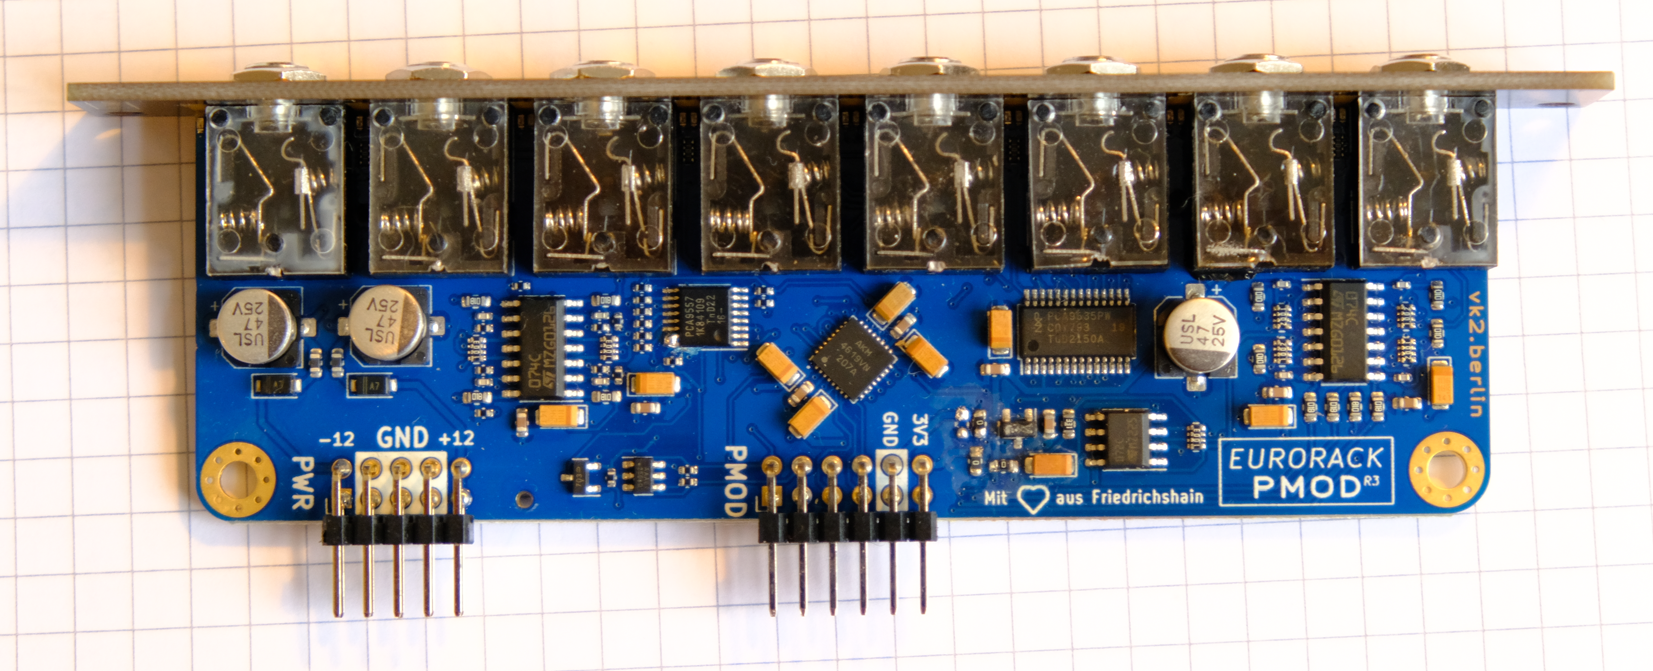
\includegraphics[height=4cm]{imgnew/pmod_top.PNG}}
\date{}

\begin{document}

\maketitle

\setwatermark{}

% OUTLINE

% why eurorack?
% why eurorack-pmod?
% evolution, how it works
% (no hardware!) sim vcv & sim testbenches
% (interest?) revision 3 and manufacturing
% stay creative

% What is Eurorack?
% Simple Eurorack system (emph. DC/CV + Audio same jacks, requirements)
% Existing FPGA-based modules (v short)
% & existing development platforms (v short)

% What is EURORACK-PMOD
% Connect to any FPGA development board like such
% Lets you write simple Verilog and explore sound
% Examples in the repository (etc...)
% Specific example

% How does this work?

% INTERESTING THINGS
% HARDWARE
% - AK4619
% - Hardware evolution
% - DC coupling & calibration
%   - Misused. Price point. Fortunately outputs are DC coupled (register allows misuse)!
% - Latency
% - Light bleed mechanism
% - Revision 3
% GATEWARE
% - Simple example cores / demo
% SIMULATION
% - VCVRack demo
% - Test benches

% CUSTOM PICS/VIDS NEEDED
% - My eurorack system
% - ICEbreaker and connected to ICEbreaker
% - Latency on scope
% - Prototypes r1 2 and 3 (next to each other?)
% - VCVrack screen capture
% - 2x video demos

% TIMING issues and bad code can be musically interesting

%   \begin{frame}{Outline}
%       % BRIEF: who am I? / side project
%       \begin{itemize}
%           \item What is Eurorack?
%           \item Why \texttt{eurorack-pmod}?
%           \item Writing \& simulating gateware
%           \item Hardware details
%           \item Interest, manufacturing \& rev. 3
%       \end{itemize}
%   \end{frame}

\begin{frame}{What is eurorack?}
    % INSERT PICTURE (my system)
    \begin{center}
        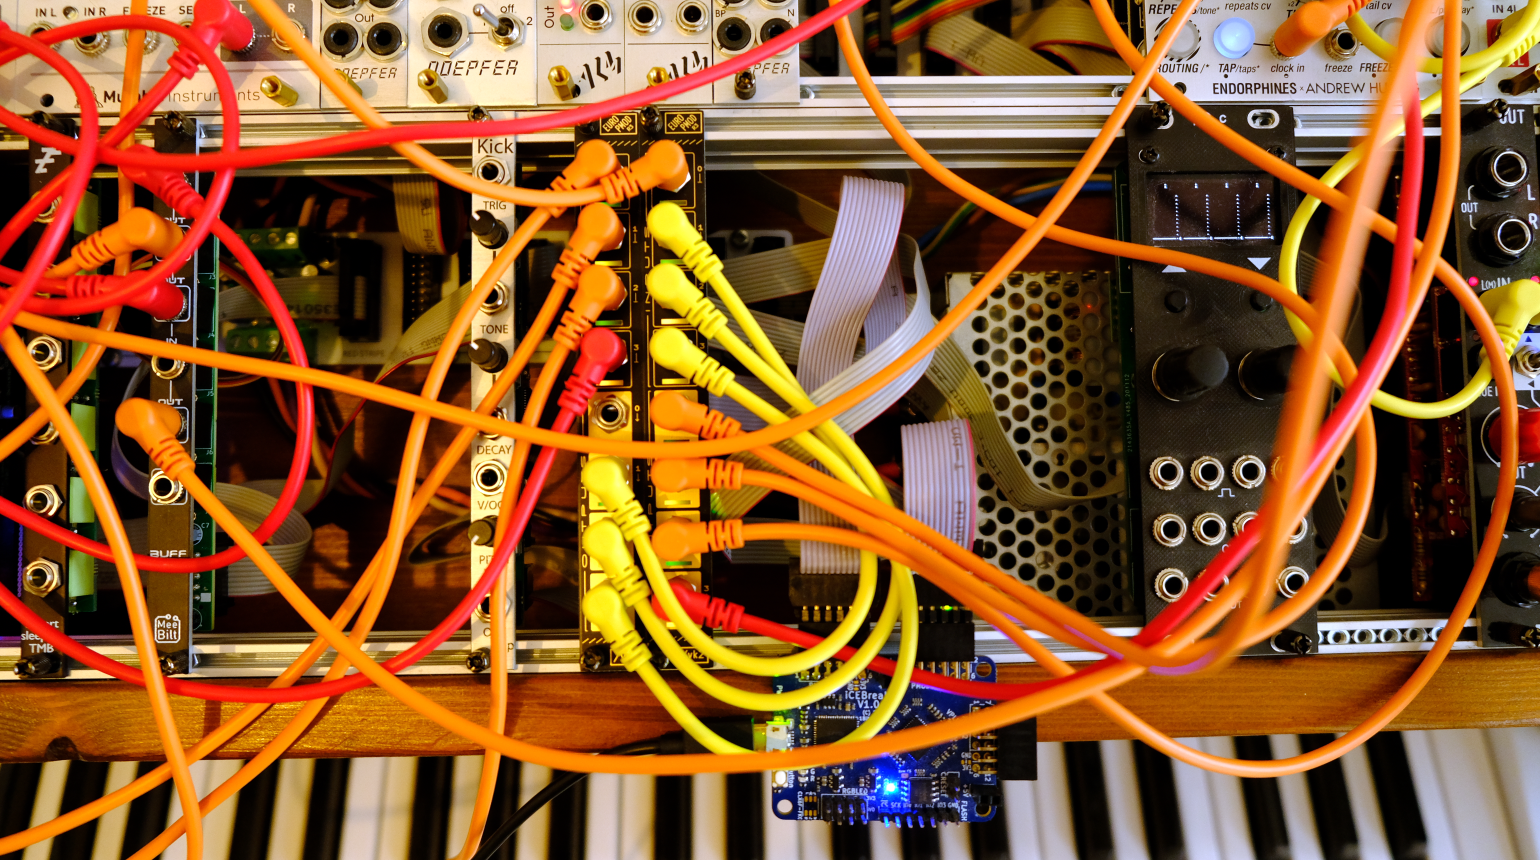
\includegraphics[height=6cm]{imgnew/pmod_insystem.png}
    \end{center}
    \begin{itemize}
        \item Modular system for constructing synthesizers.
        \item $>15,000$ modules, $>1,000$ different manufacturers.
    \end{itemize}
    % Routed manually by mono 3.5mm TS phono jacks
\end{frame}

\begin{frame}{A typical module}
    \begin{figure}
       \centering
       \raisebox{-0.5\height}{\includegraphics[height=3cm]{img/plaits_jacks.png}}
       \hspace{1cm}
       \raisebox{-0.5\height}{\includegraphics[height=3cm]{img/phono.png}}
    \end{figure}
    \begin{itemize}
        \item Modules have \textbf{input} and \textbf{output} jacks.
        \item Maximum $\pm$10V signals on \textbf{$3.5$mm mono jacks}
    \end{itemize}
    % INSERT PICTURE (module close-up with connector)
\end{frame}

\begin{frame}{}
    \begin{center}
        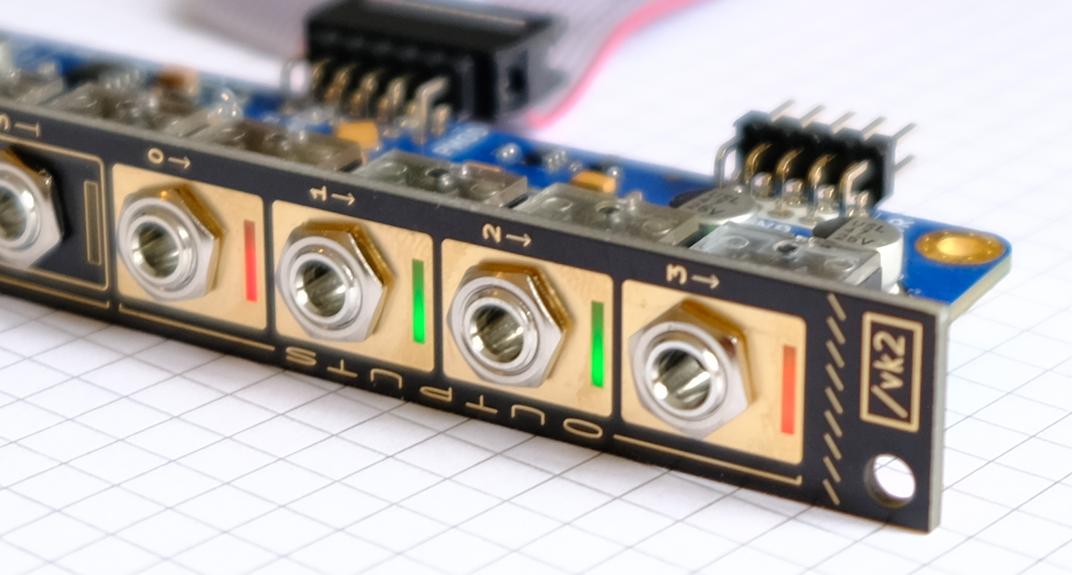
\includegraphics[height=3cm]{imgnew/leds_front.PNG}
    \end{center}
    % The hard work is already done.
    \begin{block}{Motivation}
        \begin{itemize}
            \item Easy way to get started with FPGAs \& audio synthesis.
            \item \textbf{Eurorack}: de facto standard (modular synthesis hardware).
            \item \textbf{PMOD interface}: de facto standard (FPGA dev board expansion).
            % Couldn't find anything that combines these 2 worlds.
        \end{itemize}
    \end{block}
    \begin{block}{This project}
        \begin{itemize}
            \item Open hardware design for eurorack-compatible PMOD.
            \item Open gateware design with drivers / calibration / examples.
            \item Testbenches + simulation so you can play even without hardware.
        \end{itemize}
    \end{block}
\end{frame}

\begin{frame}{iCEBreaker (from 1BitSquared) / PMOD}
    \begin{center}
        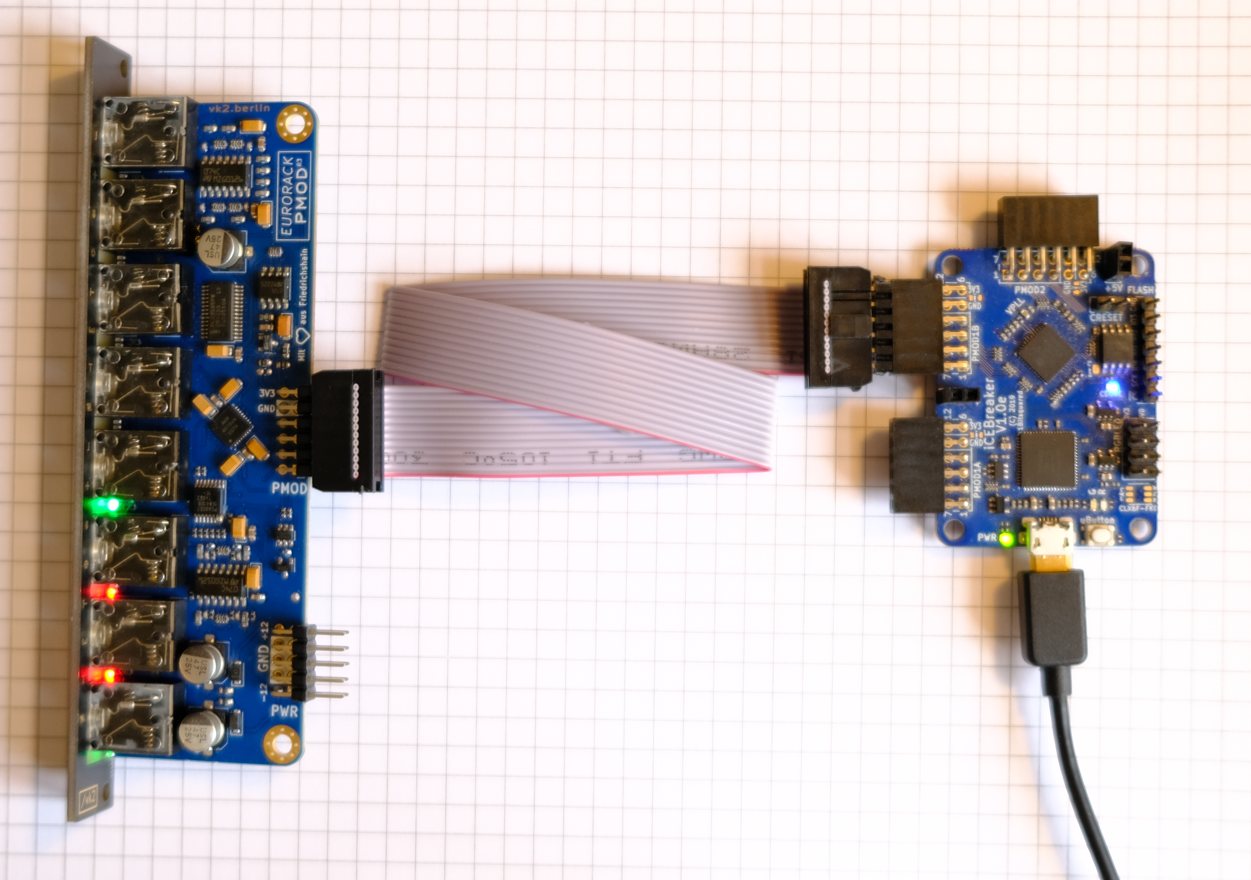
\includegraphics[height=6cm]{imgnew/pmod_top_with_icebreaker.PNG}
    \end{center}
\end{frame}

\begin{frame}{Gateware examples in \texttt{eurorack-pmod} repository}
    \begin{itemize}
        \item \texttt{vca.sv}: voltage controlled amplifier
        \item \texttt{vco.sv}: voltage controlled (wavetable) oscillator
        \item \texttt{stereo\_echo.sv}: digital echo / delay
        \item \texttt{pitch\_shift.sv}: audio rate pitch shifter
        \item \texttt{sampler.sv}: simple .wav file sampler
        \item \texttt{filter.sv}: high-pass, low-pass filter
        \item \texttt{clkdiv.sv}: clock divider
        \item \texttt{seqswitch.sv}: sequential routing switch
        \item \texttt{bitcrush.sv}: sample bit depth reducer
    \end{itemize}
\end{frame}

\begin{frame}[fragile]

    \textbf{Voltage-Controlled Amplifier (SystemVerilog)}

    \begin{minted}[highlightlines={10},highlightcolor=yellow]{verilog}
module vca #(
    parameter W = 16
)(
    input signed [W-1:0] sample_in0,
    ...
    output signed [W-1:0] sample_out0,
    ...
);

assign sample_out0 = (sample_in0 * sample_in1) >>> W;

endmodule
    \end{minted}

\end{frame}

% Blah blah blah using DMA this would be difficult

\begin{frame}{Chasing latency}
    % INSERT picture of input to output latency
    \begin{center}
        \includegraphics[height=5.5cm]{img/latency_scope1.png}
    \end{center}
    \begin{itemize}
        \item \texttt{eurorack-pmod}: about 120uS latency (24 samples @ 192KHz)
        \begin{itemize}
            \item Likely internal CODEC filter or DAC/ADC pipelining.
        \end{itemize}
        \item also pictured: \texttt{disting mk3} (digital precision adder)
    \end{itemize}
\end{frame}

\begin{frame}{Hardware overview}
    % INSERT PICTURE (hardware: top down, maybe labeled)
    \begin{center}
        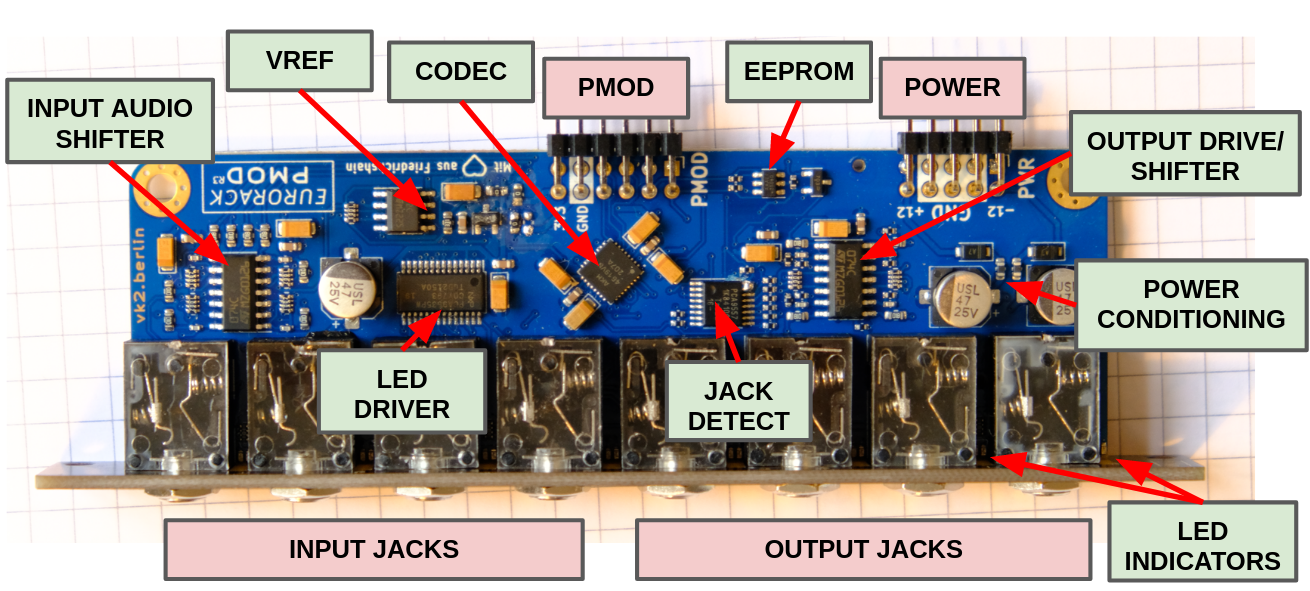
\includegraphics[height=5cm]{imgnew/labelled.png}
    \end{center}
    \begin{itemize}
        \item 3HP eurorack-compatible module with PMOD interface.
        \item 8 (4 in + 4 out) DC-coupled channels, 192KHz / 32bit capable.
        \item \textbf{NEW in R3!} Programmable LEDs // Jack detection // Calibration EEPROM
    \end{itemize}
\end{frame}

\begin{frame}{Hardware evolution}
    % INSERT 3 generations
    \begin{center}
        \includegraphics[height=5cm]{img/oldrevs.png}
    \end{center}
    \begin{itemize}
        \item KiCAD files available on GitHub.
        \item Rev. 3.1 (in production) works without any bodges.
    \end{itemize}
\end{frame}

\begin{frame}{Deeper - Audio CODEC}
    % INSERT AK4619VN datasheet capture
    % OR INSERT schematic capture
    \begin{center}
        \includegraphics[height=4cm]{img/ak4619_chip.png}
    \end{center}
    \begin{block}{AK4619VN audio codec IC}
        \begin{itemize}
            \item All 8 channels on a single I2S-like interface (fits in 1x PMOD)
            \item Much cheaper than instrumentation-quality ADCs/DACs (\$3/unit)
            \item \textbf{Can be misused in a DC-coupled mode, if calibration used}
        \end{itemize}
    \end{block}
\end{frame}

\begin{frame}{DC coupling and calibration}
    % INSERT compare input topology
    \begin{itemize}
        \item Ignore recommended input/output topology from datasheet
        \item Disable all digital high-pass filters in CODEC registers
        \item Calibrate DC extents at $\pm$ 5V, linear regression
        \item Calibrate all samples online in FPGA gateware
        % script is provided to do this (but ideally would do during mfg.)
    \end{itemize}
    \begin{center}
        \includegraphics[height=4cm]{img/datasheet_ac_coupling.png}
    \end{center}
\end{frame}

\begin{frame}{No hardware? - VCVRack}
    \begin{center}
        \includegraphics[height=5cm]{img/vcvrack.png}
    \end{center}
    \begin{itemize}
        \item VCVRack plugin to \textbf{simulate verilog on a \texttt{eurorack-pmod} module}.
        \item \texttt{github.com/schnommus/verilog-vcvrack}
    \end{itemize}
\end{frame}

\begin{frame}{Thank you for listening!}

    \begin{center}
        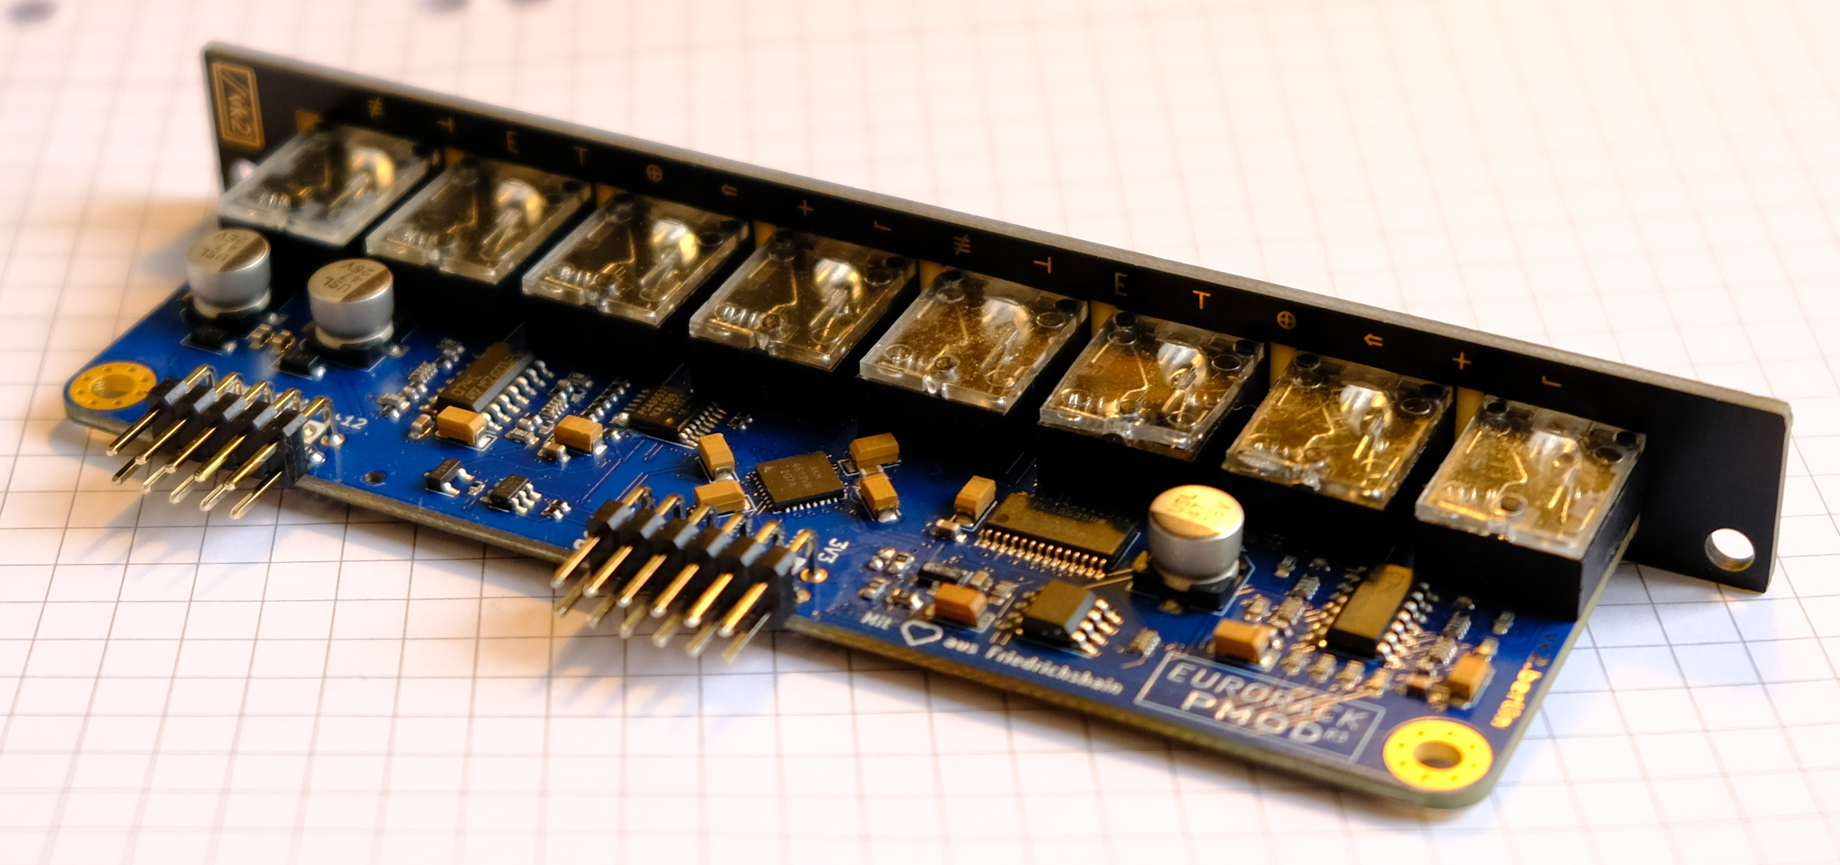
\includegraphics[height=3cm]{imgnew/pmod_backright.PNG}
    \end{center}

    \begin{itemize}
        \item contact: \texttt{me@sebholzapfel.com}
        \item \texttt{github.com/schnommus/eurorack-pmod}
        \item \texttt{github.com/schnommus/verilog-vcvrack}
    \end{itemize}

    \begin{block}{Want one? Talk to me :)}
        \begin{itemize}
            \item Star the GitHub repository
            \item Sign up in `Manufacturing' section of \texttt{README.md}
        \end{itemize}
    \end{block}

    \begin{itemize}
        \item Huge thanks to YosysHQ / 1BitSquared / everyone making open-source FPGA toolchains / platforms possible.
    \end{itemize}
    % Thank you to Icestorm / Yosys / 1BitSquared / Silvain Munaut.

\end{frame}

\end{document}
